\documentclass[border=10pt,tikz]{standalone}
\usepackage{tikz}
\usepackage{lmodern}
\usetikzlibrary{arrows.meta,positioning}

\begin{document}
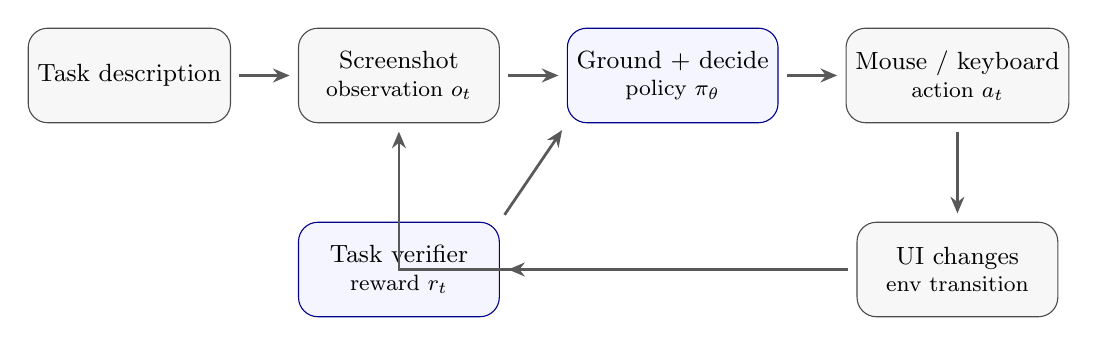
\begin{tikzpicture}[
  box/.style={draw=black!70,fill=black!3,rounded corners=7pt,minimum width=2.55cm,minimum height=1.2cm,align=center,font=\small},
  accent/.style={draw=blue!55!black,fill=blue!4,rounded corners=7pt,minimum width=2.55cm,minimum height=1.2cm,align=center,font=\small},
  arrow/.style={-{Stealth[length=6pt,width=5pt]},line width=1pt,black!65,shorten >=3pt,shorten <=3pt}
]
\node[box] (task) {Task description};
\node[box,right=0.85cm of task] (screen) {Screenshot\\[-1pt]{\footnotesize observation $o_t$}};
\node[accent,right=0.85cm of screen] (policy) {Ground + decide\\[-1pt]{\footnotesize policy $\pi_\theta$}};
\node[box,right=0.85cm of policy] (action) {Mouse / keyboard\\[-1pt]{\footnotesize action $a_t$}};
\node[box,below=1.25cm of action] (env) {UI changes\\[-1pt]{\footnotesize env transition}};
\node[accent,below=1.25cm of screen] (verify) {Task verifier\\[-1pt]{\footnotesize reward $r_t$}};
\draw[arrow] (task) -- (screen);
\draw[arrow] (screen) -- (policy);
\draw[arrow] (policy) -- (action);
\draw[arrow] (action) -- (env);
\draw[arrow] (env) -- (verify);
\draw[arrow] (env.west) -| (screen.south);
\draw[arrow] (verify.north east) -- (policy.south west);
\end{tikzpicture}
\end{document}
